%%%%%%%%%%%%%%%%%%%%%%%%%%%%%%%%%%%%%%%%%%%%%%%%%%%%%%%%%%%%%
%% GENERELLE EINSTELLUNGEN
%%%%%%%%%%%%%%%%%%%%%%%%%%%%%%%%%%%%%%%%%%%%%%%%%%%%%%%%%%%%%	

%dokumentenklasse
\documentclass[a4paper,oneside,12pt,titlepage,chapterprefix]{scrreprt}

%packages
\usepackage[english]{babel}
\usepackage[T1]{fontenc}
\usepackage[utf8]{inputenc}
\usepackage{lmodern} 
\usepackage{graphicx}
\usepackage{setspace}
\usepackage{fancyhdr}
\usepackage[header=plain, number=none, toc=true]{glossary}
\usepackage{url}
\usepackage{booktabs}
\usepackage{paralist}
\usepackage{enumitem}
\usepackage[bookmarksnumbered=true]{hyperref}
\usepackage{color}
\usepackage{listings}
\usepackage{floatflt}
\usepackage{geometry}
\usepackage{pdfpages}
\usepackage{prettyref}
\usepackage{caption}
\usepackage{subcaption}
\usepackage{wrapfig}
\usepackage{abstract}

%r�nder anpassen
\geometry{a4paper, top=28mm, left=27mm, right=26mm, bottom=30mm, headsep=8mm, footskip=12mm}

%farben f�r den text (listings definieren)
\definecolor{darkblue}{rgb}{0,0,.5}
\definecolor{wine}{rgb}{0.53,0.047,0.047}
\definecolor{lightgray}{rgb}{.2,.2,.2}
\definecolor{darkgreen}{rgb}{0,.4,0}

\hypersetup{colorlinks, pdfauthor={Tom Bullmann, Andreas N\"u\ss{}lein, Sebastian Schulz, Mareike Ziese},
	pdftitle={TaWusel},
	pdfnewwindow=true, linkcolor=black, citecolor=black,
	filecolor=darkgreen, urlcolor=blue}

%formatierung der listings
\renewcommand{\lstlistingname}{Code listings}
\lstset{
	tabsize=2,
	%kleine schriftgr��e
	basicstyle=\footnotesize \bfseries\ttfamily,
	keywordstyle=\color{wine},
	identifierstyle=\mdseries \color{black},
	commentstyle=\itshape\mdseries\color{darkgreen},
	stringstyle=\ttfamily,
	showstringspaces=false,
	stringstyle=\color{darkblue},
	%chars to escape inline = (*this is escaped*)
	escapeinside={(*@}{@*)},
	language=Java
}

\lstset{
	numbers=left,
	numberstyle=\scriptsize,
	stepnumber=1,
	numbersep=5pt
}

\lstset{
	captionpos=t,
	frame=single,
	frameround=tttt,
	breaklines=true,
	breakatwhitespace=true,
	showlines=true,
}

\lstset{
	emph={logger,
		properties,
		dbConnection,
		instance
	},
	emphstyle= {\itshape \color{darkblue}},
}


%variablen
\newcommand{\code}[1]{{\small\ttfamily #1}}
\newcommand{\codeCap}[1]{\textsc{\small #1}}

\begin{document}

	%kopf- und fu�zeilen
	\setlength{\headheight}{28pt}
	\pagestyle{fancy}
	\fancyhf{}
	\lhead{Team 1}
	\chead{\textbf{SWP: Client project II - Web technologies} \\ Lecturer: Prof. Dr. M\"uller-Birn}
	\rhead{SS 12 \\ \today}
	\cfoot{\tiny{Free University of Berlin\\ Department of Mathematics and Computer Science\\
Institute of Computer Science}}	
	\rfoot{\smallskip \thepage}
	\renewcommand{\footrulewidth}{0.4pt} %untere Trennlinie

	%kopf und fu�zeilen f�r alle seiten (auch inhalt und anhang)
	\fancypagestyle{plain}{
    \fancyhf{}
		\lhead{Team 1}
		\chead{\textbf{SWP: Client project II - Web technologies} \\ Lecturer: Prof. Dr. M\"uller-Birn}
		\rhead{SS 12 \\ \today}
		\cfoot{\tiny{Free University of Berlin\\ Department of Mathematics and Computer Science\\ Institute of Computer
Science}}	
		\rfoot{\smallskip \thepage}
		\renewcommand{\footrulewidth}{0.4pt} %untere Trennlinie	
	}

	\renewcommand{\chaptermark}[1]{\markboth{\thechapter.\ #1}{}}
	\newcommand{\emptyRow}{\medskip \noindent}


	%r�mische bezifferung
	\pagenumbering{Roman}
	\setcounter{page}{0}


%%%%%%%%%%%%%%%%%%%%%%%%%%%%%%%%%%%%%%%%%%%%%%%%%%%%%%%%%%%%%
%% VORBEMERKUNGEN & VERZEICHNISSE
%%%%%%%%%%%%%%%%%%%%%%%%%%%%%%%%%%%%%%%%%%%%%%%%%%%%%%%%%%%%%	

	%deckblatt
	\begin{titlepage}
  \begin{center}
    \Large
    \textsc
    {
    	\\
    	\vspace{2cm}
    	Softwareprojekt: Kundenprojekt II \\ Webtechnologien
    }\\
  	\vspace{5cm}
  	\textsc
  	{
  		Gruppendokumentation\\[0.5\baselineskip]
  		von\\[0.5\baselineskip]
  		Team 1\\
		\begin{tiny}
			Tom Bullmann\hspace{1cm}Andreas N\"u\ss{}lein\hspace{1cm}Sebastian Schulz\hspace{1cm}Mareike Ziese\\
		\end{tiny}
  	}
  	\vspace{5cm}
    \textsc{\today}\\
    \vspace{1cm}
    \textsc
    {
    	Dozentin:\\
    	Prof. Dr. M\"uller-Birn
    }\\
  	\vspace{1cm}
  	\normalsize
  	\textsc{
  		Freie Universit\"at Berlin\\
  		Fachbereich Mathematik und Informatik\\
  		Institut f\"ur Informatik
  	}\\
  \end{center}
\end{titlepage}

	%inhaltsverzeichnis
	\clearpage
	\addcontentsline{toc}{chapter}{Table of contents} 
	\tableofcontents

	%abbildungsverzeichnis
	\clearpage
	\addcontentsline{toc}{chapter}{Table of figures}
	\listoffigures

	\clearpage

	%abstand im inhaltsverzeichnis
	\addtocontents{toc}{\protect\vspace*{0.6\baselineskip}}
	
%%%%%%%%%%%%%%%%%%%%%%%%%%%%%%%%%%%%%%%%%%%%%%%%%%%%%%%%%%%%%
%% HAUPTTEIL
%%%%%%%%%%%%%%%%%%%%%%%%%%%%%%%%%%%%%%%%%%%%%%%%%%%%%%%%%%%%%

	%seiten in arabisch durchnummerieren
	\clearpage
	\pagenumbering{arabic}
	\setcounter{page}{1}

	%einleitung
	%introduction
\renewcommand{\abstractname}{Introduction}
\begin{abstract}
The sole purpose of this document is to describe the complete process of the project, which was done in the cooperation of the
Carmeq GmbH and the Free University of Berlin, with the topic of intermodal passenger transportation.

\emptyRow
At the beginning of this course there were 18 students enrolled for this course. They have been divided into 4 teams, which
worked separately from the beginning.
\end{abstract}

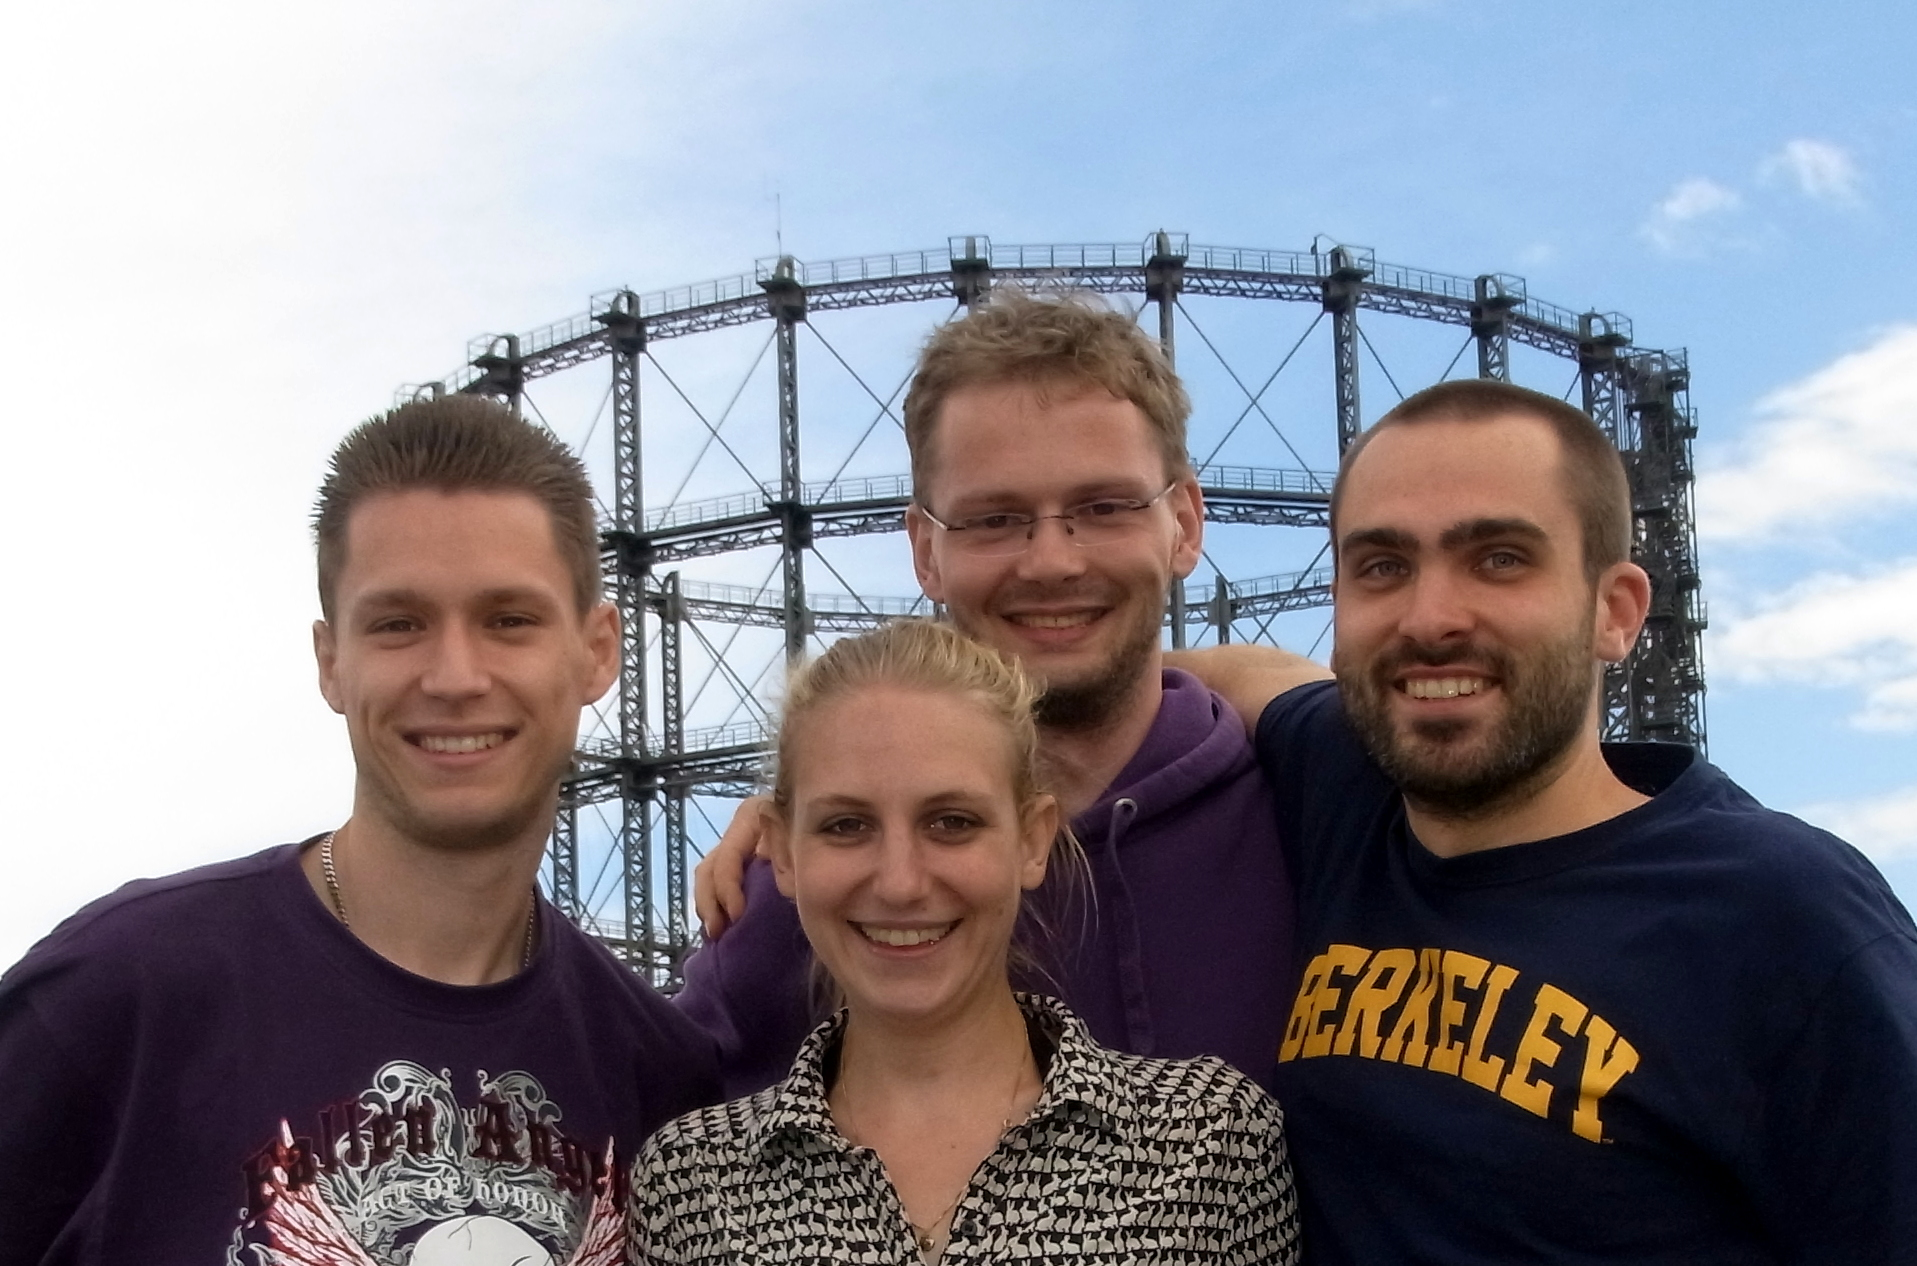
\includegraphics[width=\textwidth]{images/team1.jpg}
\clearpage

	%anforderungsanalyse
	\chapter{Requirement engineering}\label{chp:ReqE}
	%requirement engineering

	%Modellierung
	\chapter{Modeling}\label{chp:Mod}
	%modeling

\section{persona}

\subsection{preparement}

After figured out the main problem it was time to use our fantasy. We should create a typical CARMEQ worker based on our results
of the interviews. This person is called 'persona'. In each phase of the development we will need him to help us to find our
target. It doesn't make sense to create a application in the intention to satisfy everybody, its better to shrink the requirements
to avoid to have in the end a program which can do a little bit of everything, where nobody knows what he can really do with. 

\subsection{implementation}

We started with 2 prototypes, one with the bahncard50 and the other with bahncard100. Finally we choosed the second because in our
opinion he has more problems on which we could have an influence. The typical CARMEQ worker is middle-aged, ambitious with a
high education level. In the reason of having the bahncard he has to travel a lot, the main reason for this is that he could work
as project manager.  We created a person named 'Batur Temel', the whole persona is shown in \prettyref{fig:persona1}, 
\prettyref{fig:persona2},  \prettyref{fig:persona3} and  \prettyref{fig:persona4}.

\clearpage

\begin{figure}[!h]
	\includegraphics[scale=0.8, page=1]{images/Persona_final.pdf}
	\caption{persona sheet 1}
	\label{fig:persona1}
\end{figure}

\clearpage

\begin{figure}[!h]
	\includegraphics[scale=0.8, page=2]{images/Persona_final.pdf}
	\caption{persona sheet 2}
	\label{fig:persona2}
\end{figure}

\clearpage

\begin{figure}[!h]
	\includegraphics[scale=0.8, trim=0mm 20mm 0mm 20mm,clip,page=3]{images/Persona_final.pdf}
	\caption{persona sheet 3}
	\label{fig:persona3}
\end{figure}

\begin{figure}[!h]
	\includegraphics[trim=0mm 240mm 0mm 20mm,clip,scale=0.8, page=4]{images/Persona_final.pdf}
	\caption{persona sheet 4}
	\label{fig:persona4}
\end{figure}

\section{point of view}

\subsection{preparement and  implementation}

The point of view helps also to clarify which requirements we want to handle. We tried to see with the eyes of our persona and
work them out. He has a problem with his payoff because of his bahncard100 usually he has no proof when he did a travel. In
addition he has also the problem with the seat reservation and the taxi-use.

\begin{figure}[!h]
	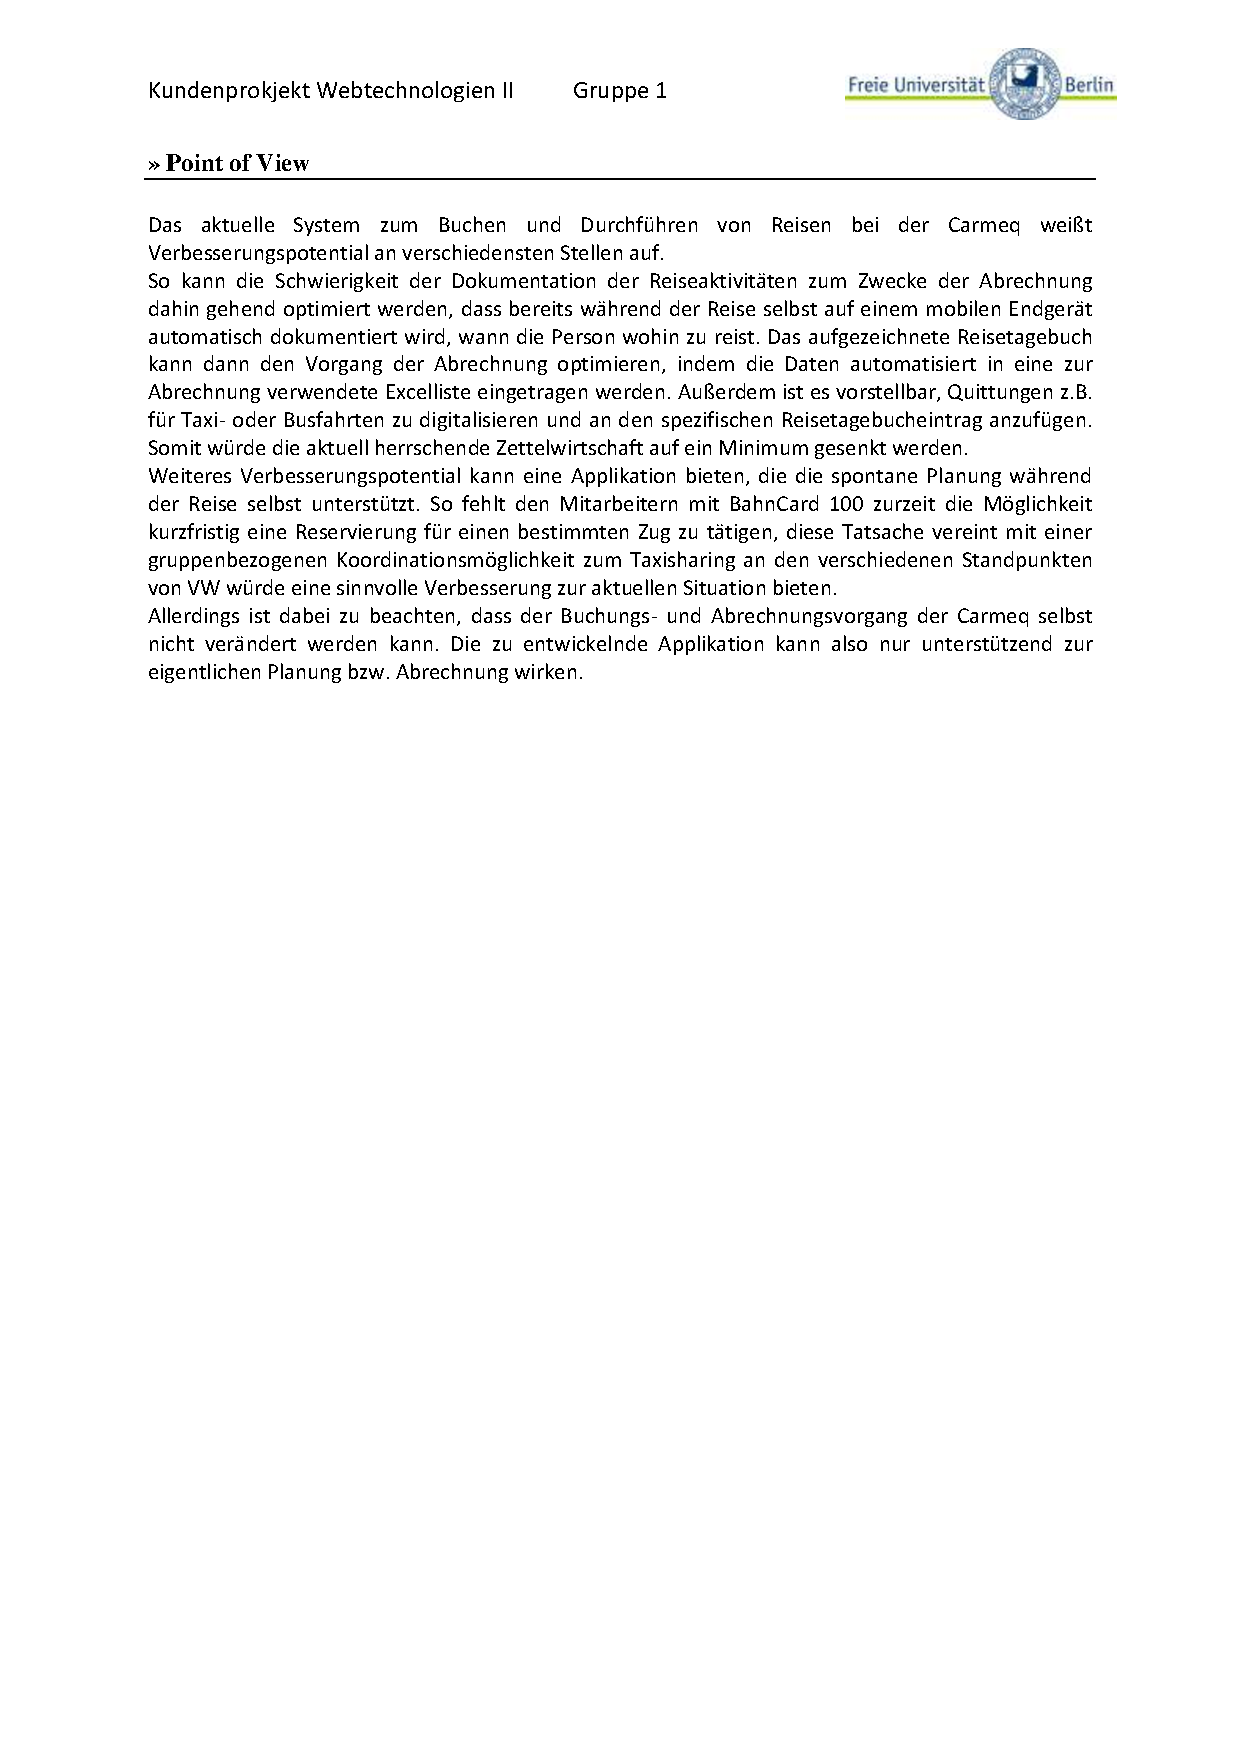
\includegraphics[trim=0mm 140mm 0mm 20mm,clip,scale=0.8, page=1]{images/POV.pdf}
	\caption{point of view}
	\label{fig:pov}
\end{figure}

\clearpage

	
		
	%conception
	\chapter{Conception}\label{chp:Conc}
	% !TEX encoding = Windows Latin 1
%conception

\section{implementation}
On the fundament of our persona and his point of view we did a lot of brainstorming to find innovative ideas to ease his traveling. We wrote everything what came to or mind on small post its and clustered it in main ideas. In the end we got 5 big nodes as you see in \prettyref{fig:conception}. At least we choose two ideas, which we presented in the kickOff. We chooses these two because we thought that they would help both factions of bahncard-users.


\begin{figure}[!h]
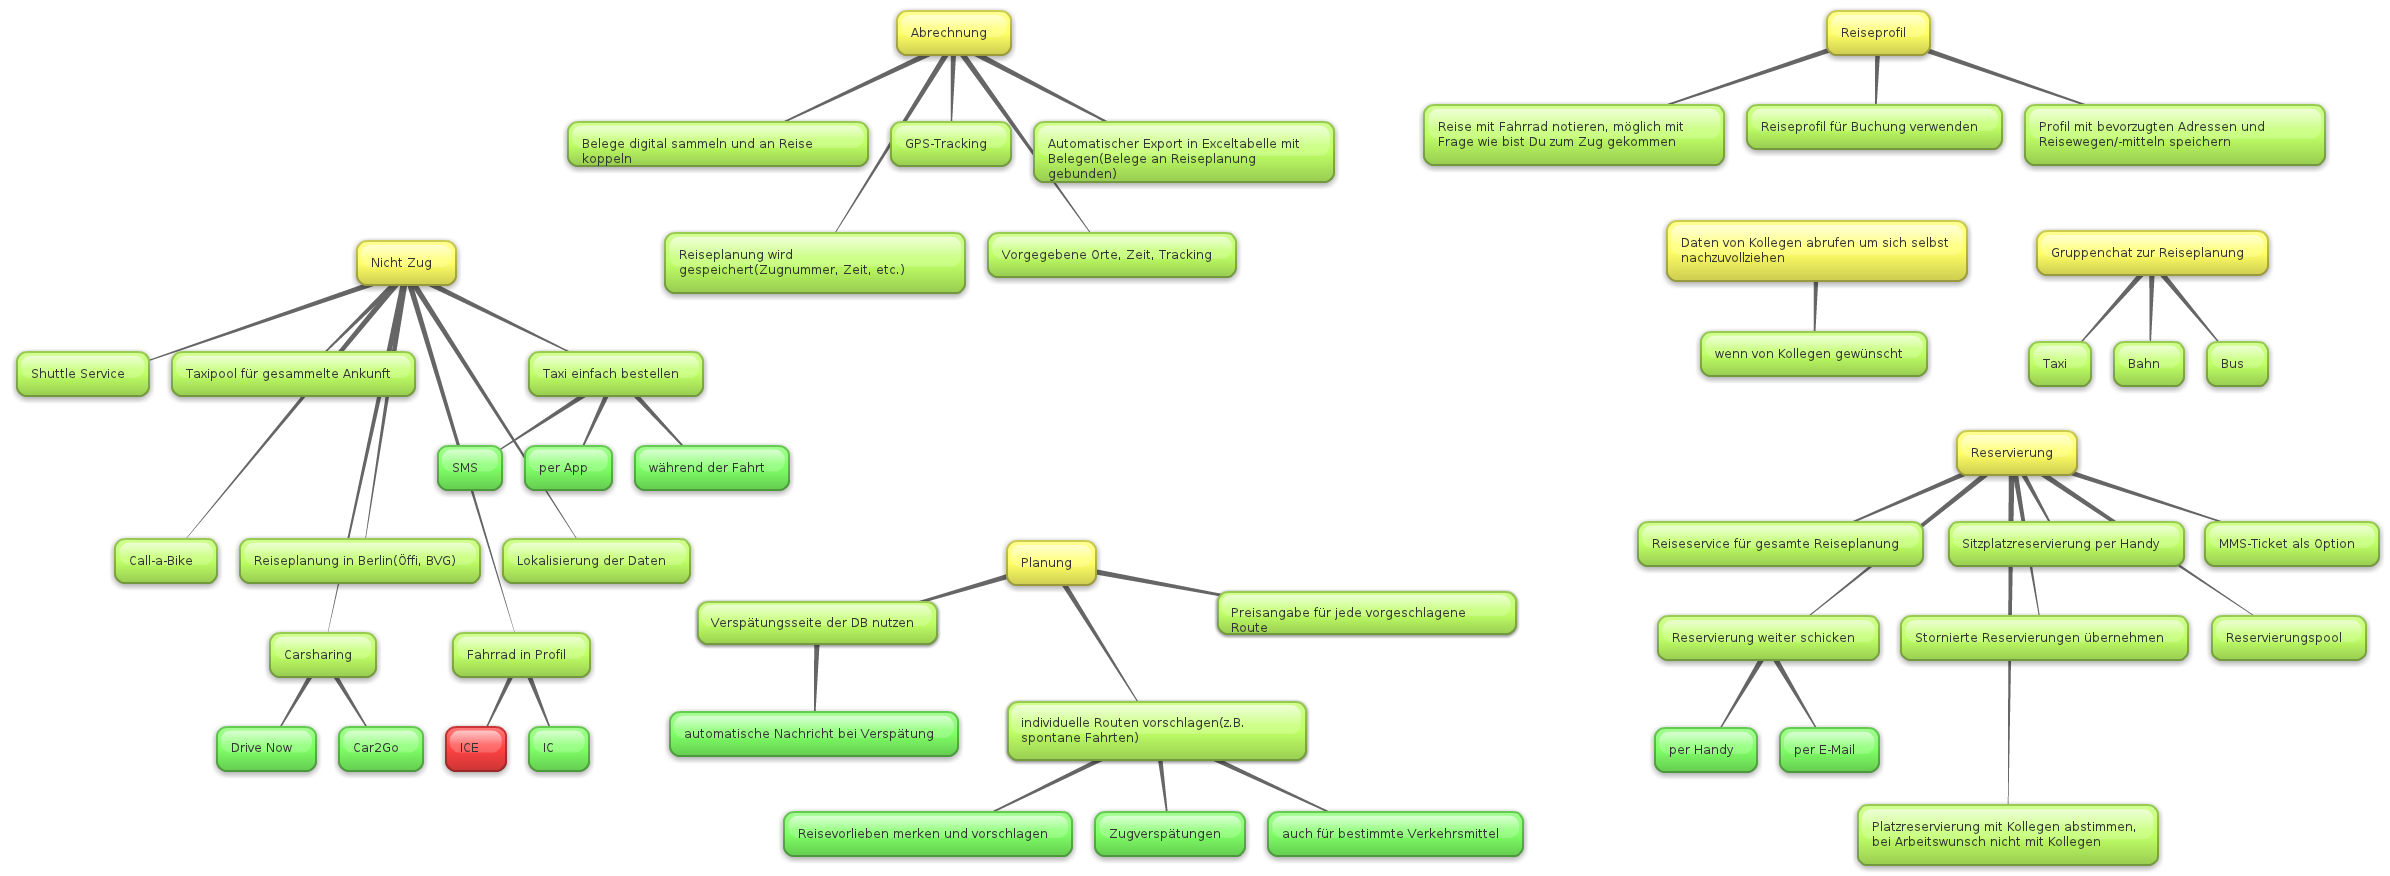
\includegraphics[width=1.0\textwidth, height=130mm]{images/konzeption.png}
\caption{conception}
\label{fig:conception}
\end{figure}
\clearpage

\section{idea 1 : taxi sharing}

In the first idea we wanted to ease the use of taxis in Wolfsburg. Often you sit  in the same train like your colleagues but you don�t know. Instead of sharing a taxi, you send more money for it and have double trouble. We wanted to create a platform where you can see who also want to take a taxi to a certain time from place A to place B. In the best case the taxi-order should be automated, so you have no stress getting your taxi punctual with no stress of searching and running(like its usually at the main line).

\section{idea 2: travel diary}

This solution should ease the payoff f the CARMEQ-workers. The application would track the position of the user and with the help of these tracks the application can calculate when the user have been traveled. At the end of each month you can use this diary to complete your own notes.


\section{decision}
 Both idea were accepted good, so its was up on us, to decide. We choose the first idea. The only reason for this decision was more interests in this theme.
 
 
	
	%paper prototype
	\chapter{Paper prototype and User Stories}\label{chp:PapP}
	%paper prototype
	
	%prototype
	\chapter{Prototype implementation}\label{chp:Prot}
	%prototype

The following chapter comprises the main activity of the project: the implementation of the TaWusel web service and the TaWusel
Android application. At the beginning we take a look at the basic architecture design of the whole service in section
\ref{sec:GArc}. Afterwards the database design is described in a brief section.

\emptyRow
Subsequently to the fundamentals the section \ref{sec:Webs} takes a closer look at the implementation of the web service.

\emptyRow
Last but not least the focus of section \ref{sec:Andr} will be on the Android application. Here you will find a brief description
of its functions (see \ref{ssec:AndrDes}), some design thoughts regarding the class diagram and a description of the classes which
are used by the app (see \ref{ssec:AndrArc}) as well as an installation guide to run the app on your mobile device (see
\ref{ssec:AndrInst}). 

\emptyRow
You can retrieve more information if you follow the link to our issue tracker
(\url{https://github.com/nutztherookie/swp_kp2_2012_gruppe1/issues}) Here most of our task which came up while the implementation
are covered. There are also some issues which are labeled with the prefix "wishlist", these are suggestions how one could improve
the service in the future. The whole document with all estimated users stories you can find in appendix \ref{chp:US}.

\clearpage

\section{General architecture}\label{sec:GArc}
%general architecture
\begin{figure}[ht]
	\centering
	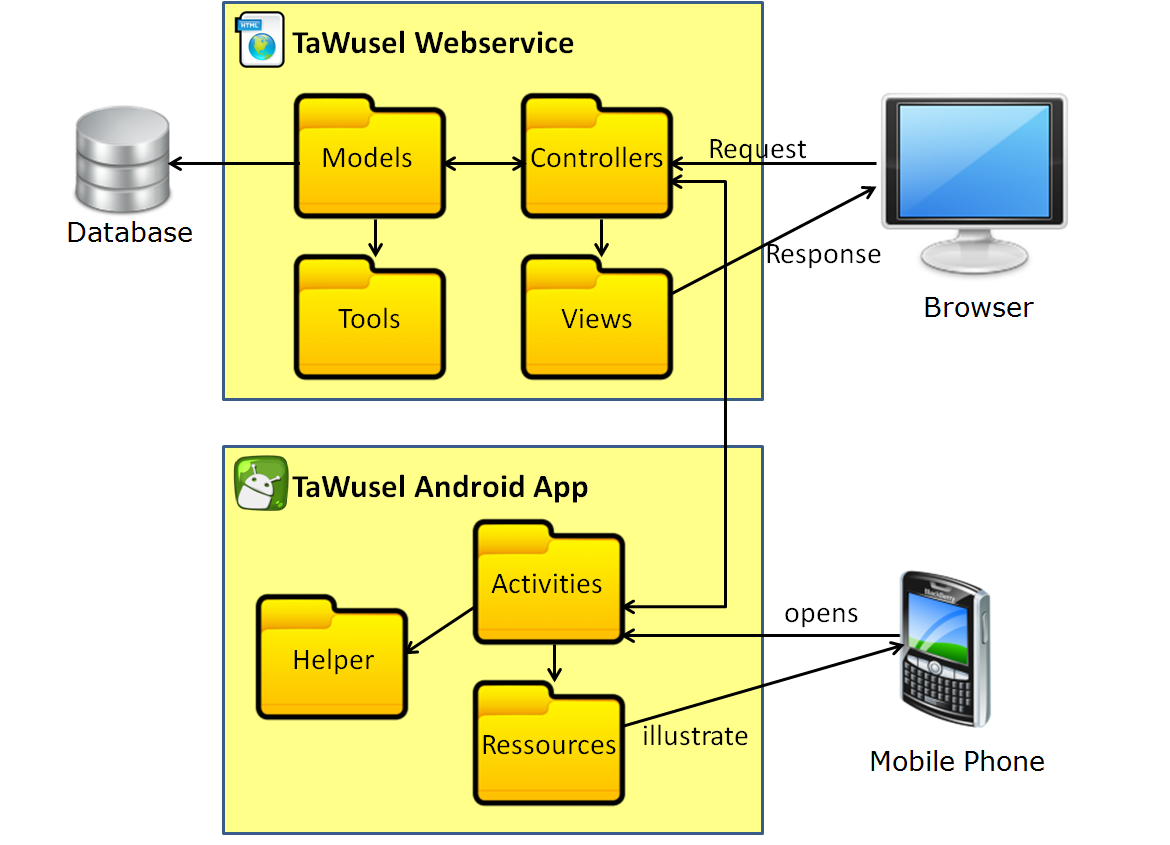
\includegraphics[width=0.8\textwidth]{images/Architekturdiagramm}
	\caption{architecture diagram}
	\label{img:Arch}
\end{figure}



\clearpage
\section{Database modeling}
%db modeling
\begin{figure}[ht]
	\centering
	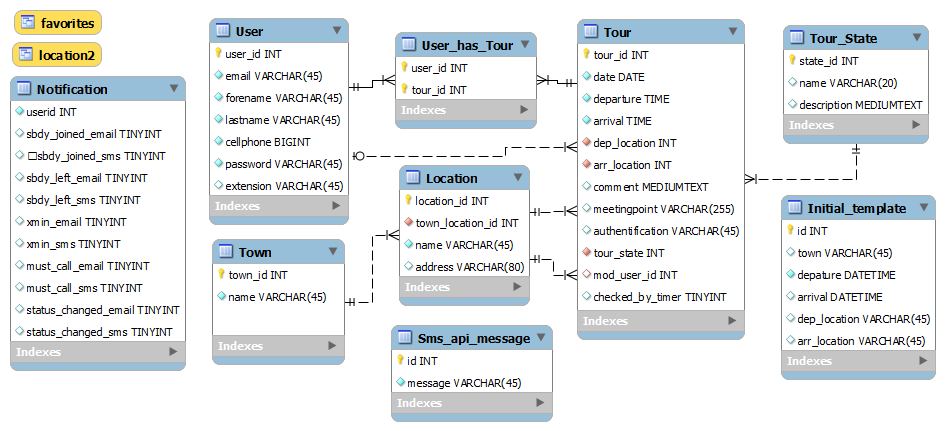
\includegraphics[width=0.8\textwidth]{images/Datenbank_Model}
	\caption{database model}
	\label{img:DBMod}
\end{figure}
Our database consists of a few tables for basic functionality, like user management or creation of a tour, and two views which
have to be used due to circumstances with play2 and its ANORM, which provides just some basic features and not the entire
capability of SQL.

\clearpage
\section{Webservice}\label{sec:Webs}
%webservice
\subsection{Description}\label{ssec:WedDesc}

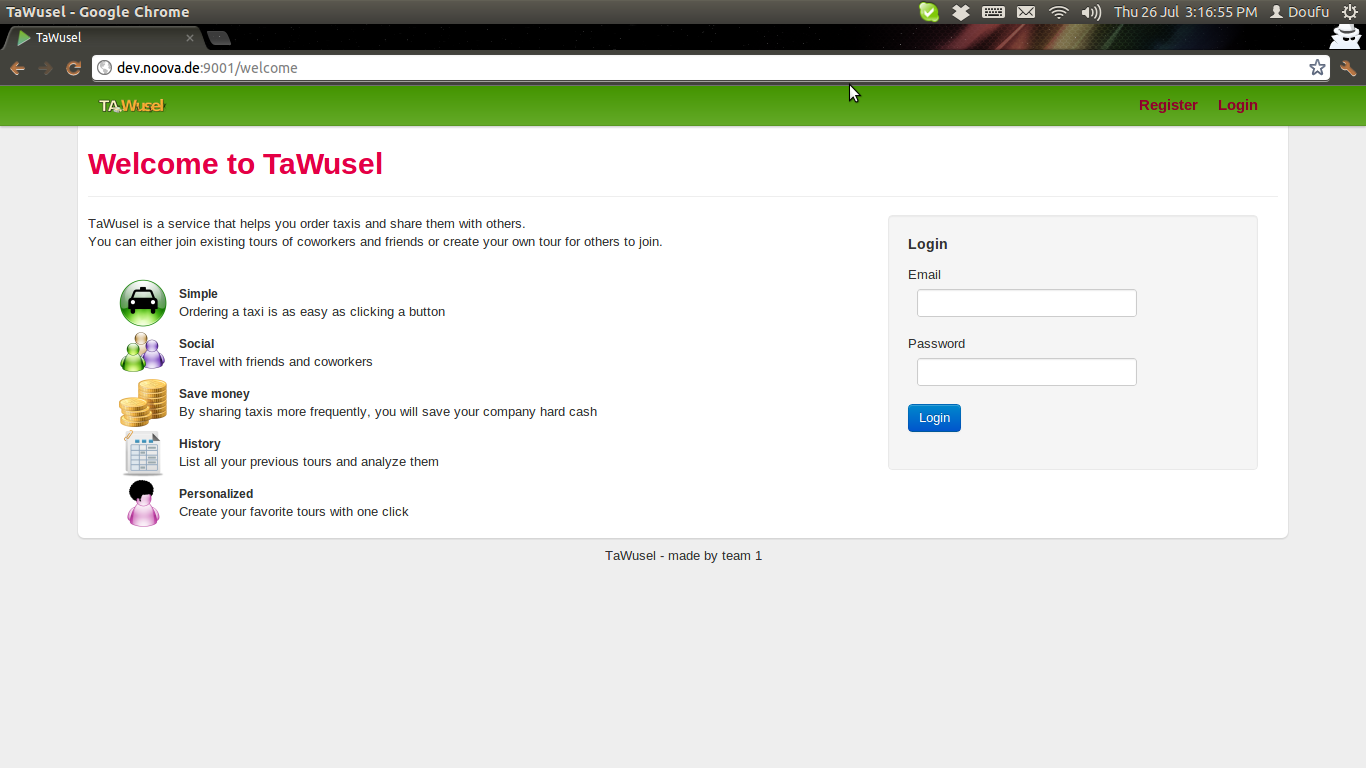
\includegraphics[width=16cm]{images/TaWusel_Web_Login.png}\label{img:WebLogin}
blabla


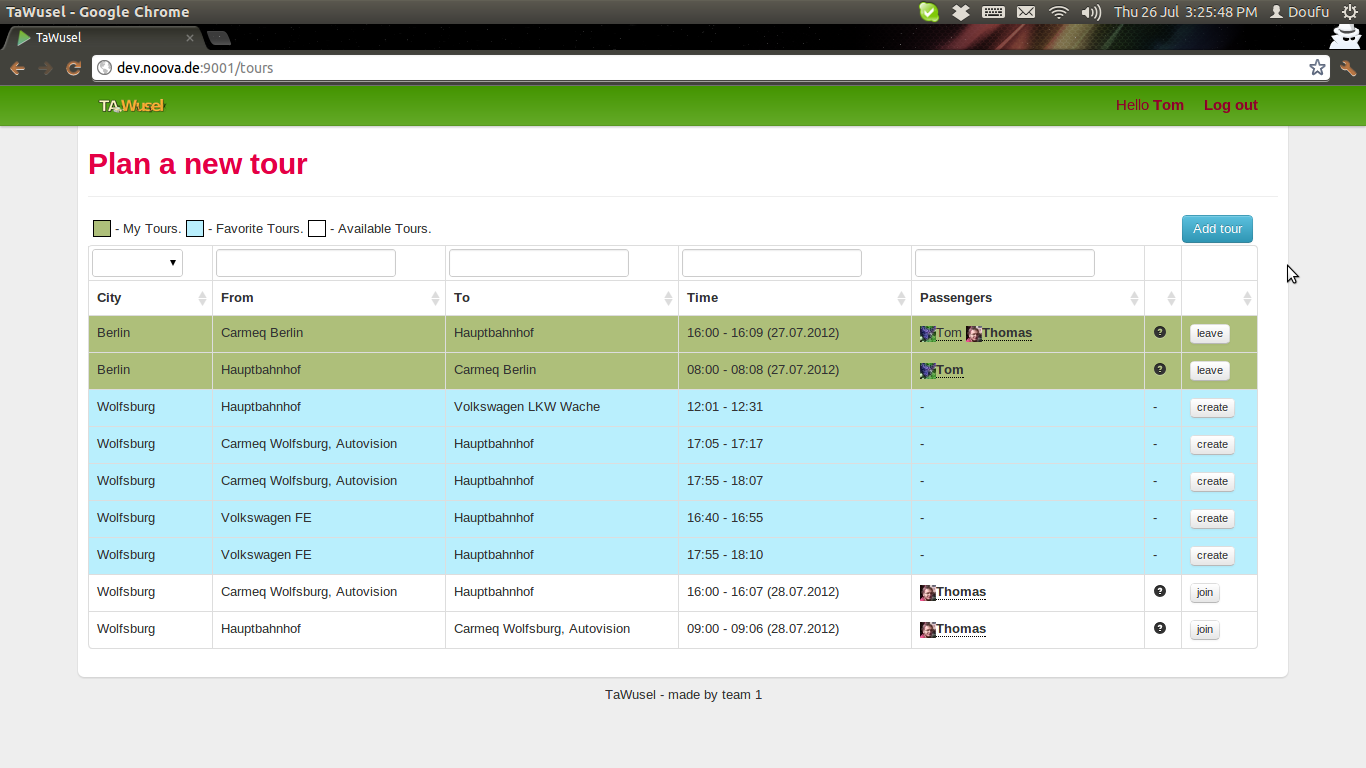
\includegraphics[width=16cm]{images/TaWusel_Web_main.png}\label{img:WebLogin}



\begin{figure}[h]
	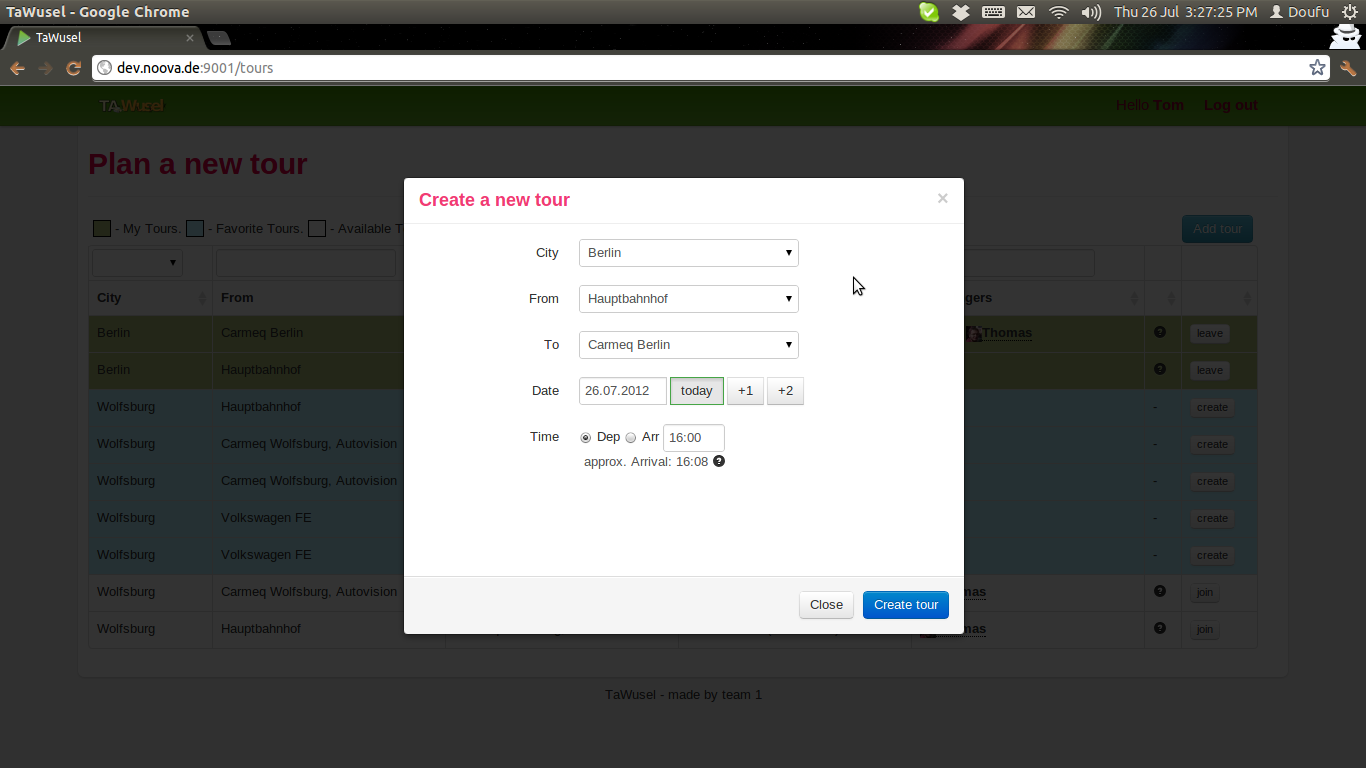
\includegraphics[width=16cm]{images/TaWusel_Web_create.png}
	\caption{modal panel for creating a tour}
	\label{img:WebLogin}
\end{figure}



\begin{figure}[h]
	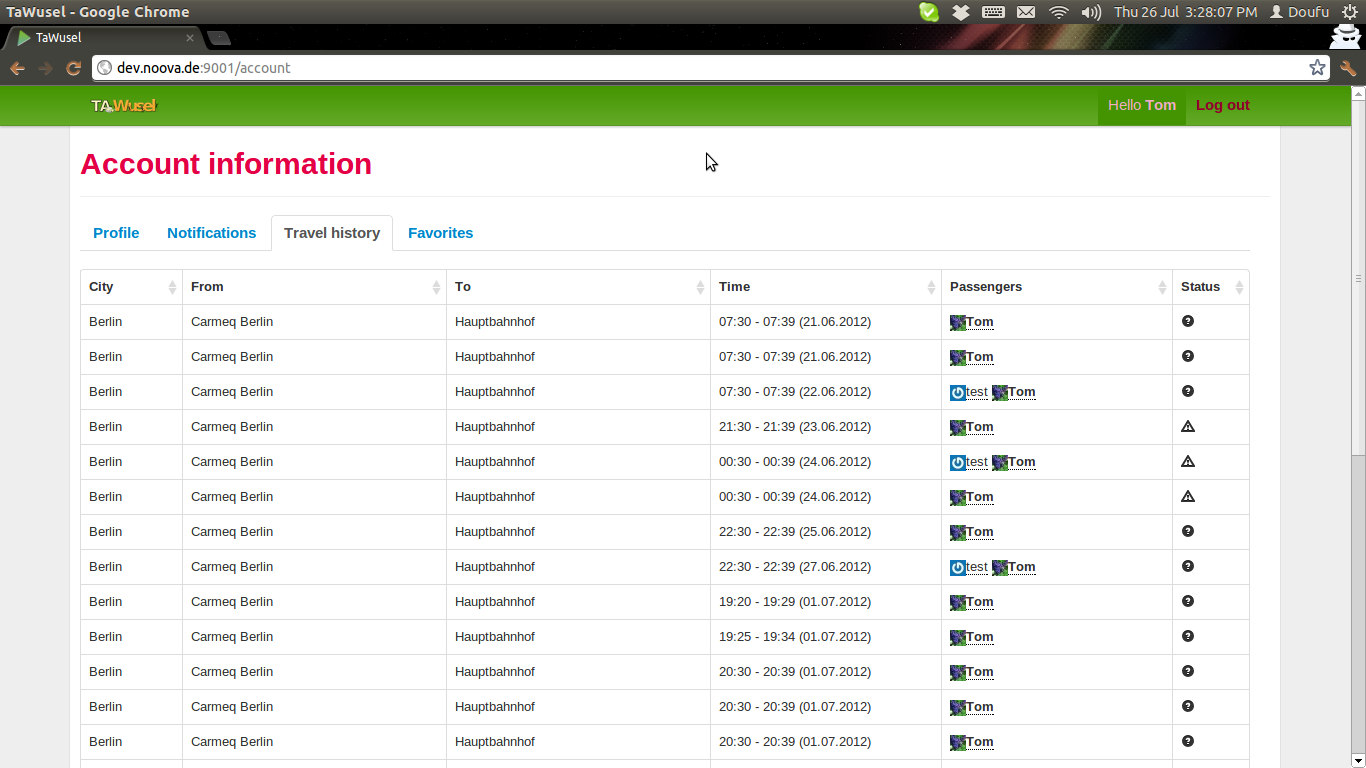
\includegraphics[width=16cm]{images/TaWusel_Web_history.png}
	\caption{profile page - history tab}
	\label{img:WebLogin}
\end{figure}
\subsection{Installation guide - Webservice}\label{ssec:WebInst}

The rough install instructions can also be found in the \texttt{INSTALL.md} file.
\begin{itemize}

\item As TaWusel uses the Play!2 framework (Scala version) obviously the first requirement is said framework. To obtain it, the
best way is to follow the official installation documentation from the Play!
website\footnote{\url{http://www.playframework.org/}}.

\item The next step is to set up a MySQL-database\footnote{In theory, other SQL-DBMS should work as well, since TaWusel uses
JDBC for its connections. However we have only used MySQL so far.} for your project.
As installing MySQL can obviously not be part of this documentation, we shall only briefly point towards the official
website\footnote{\url{http://dev.mysql.com/doc/refman/5.6/en/installing.html}} and name
XAMPP\footnote{\url{http://www.apachefriends.org/en/xampp.html}} and MAMP\footnote{\url{http://www.mamp.info}} as two easy
alternatives
for installing MySQL on Windows and Mac OS X respectively.\\
Example code for setting up the database:
\begin{verbatim}
CREATE DATABASE tawusel;
CREATE USER tawusel;
GRANT ALL ON tawusel.* TO tawusel@localhost IDENTIFIED BY 'pass';
\end{verbatim}
\small{To use other credentials, the \texttt{conf/application.conf} has to be changed accordingly.}

\item Lastly go to \url{https://github.com/nutztherookie/tawusel} and download TaWusel. Unzip, go to the project's root folder and
run \texttt{play run}.\\
Point your web browser to \url{http://localhost:9000/}


\end{itemize}

\clearpage
\section{Android App}\label{sec:Andr}
%android
\subsection{Description}\label{ssec:AndrDes}
\begin{floatingfigure}[r]{5cm}
	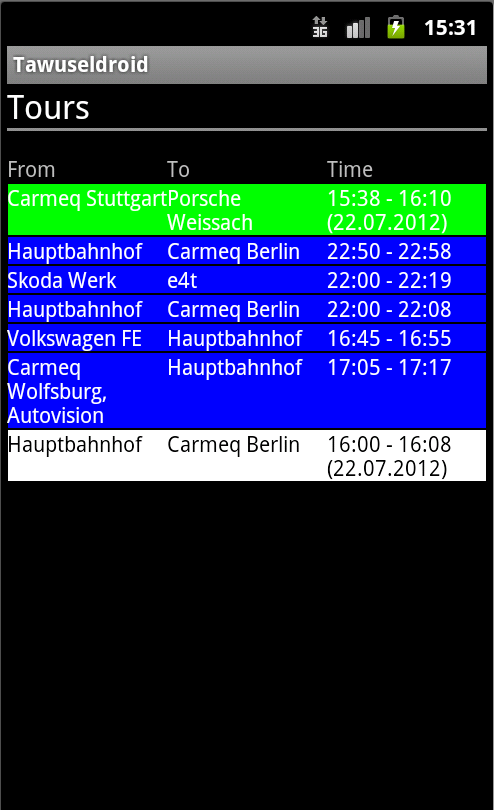
\includegraphics[width=4cm]{images/Tawuseldroid_tours.png}
	\caption{main view}
	\label{img:AndMV}
\end{floatingfigure}

\noindent
After the development of the key features of the TaWusel web service the team decided to implement an android app prototypically. This guarantees that all Carmeq employees who have access to an android phone can use the service more comfortable. The biggest advantage of an implementation of an android application is that the mobile phone doesn't need to have internet access at the whole time of the journey. On the other hand if one calls the web service with a web browser an internet connection is mandatory.

\emptyRow
The android application includes the most valuable features like creating a new tour or joining/leaving an existing tour. In figure \ref{img:AndMV} you can see the main view of the prototype. Like in the web service there is a table which is divided into three parts: the user's active tours, the templates to create a new to more comfortable and available tours created by other users. Since the application is a rough prototype the look and feel can be improved in most of the views, e.g. the colors of the tours table are just the standard android colors for green, blue and white to link their appearance to the corresponding entries in the web service.  

\emptyRow
\begin{floatingfigure}[l]{5cm}
	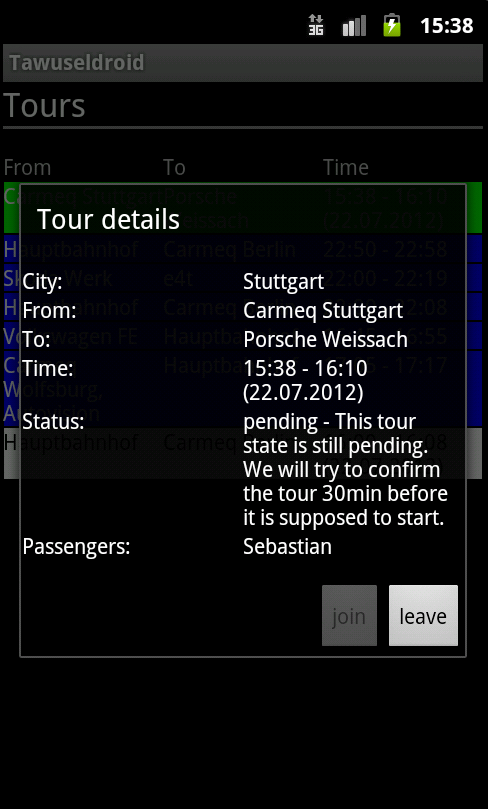
\includegraphics[width=4cm]{images/Tawuseldroid_details.png}
	\caption{details dialog}
	\label{img:AndDet}
\end{floatingfigure}
\noindent
By clicking on an existing tour a dialog is opened which shows more details according the chosen tour (see figure \ref{img:AndDet}). Here you find more information like the tour status or the passengers registered for it. For creating a new tour you can either pick a template (one of the blue rows) or click on the item "add tour" in the content menu. A dialog similar to the details dialog occurs. Here you can choose the city and the locations as well as the date and the time of the tour. To change the date as well as the departure or arrival time you just have to click on the corresponding field and a picker dialog appears.  A picture of the create dialog can be found in the appendix A in figure \ref{img:AndCD}.

\emptyRow
Unfortunately in the short period of development we were not able to implement a push function in the web service. So you have to fetch the tour data manually. For that reason just click on the item "update data" in the content menu. Remember that the mentioned activities call methods from the web service, therefore you need to have internet access.

\clearpage
\subsection{Architecture}\label{ssec:AndrArc}



\subsection{Installation guide}\label{ssec:AndrInst}

\begin{enumerate}
	\item Make sure you locate the tawusel.properties into the assets folder. Here you have to replace the json server property ("http://10.0.2.2:9000/") by the address of the server your tawusel service is running on.
	\item Generate your tawusel.apk. You can directly generate the apk from your eclipse project.
	\item Install the apk on your mobile phone.(Remark: the current version works stable on android 2.3.3 but its working on higher versions is not guaranteed)
\end{enumerate}



	
%%%%%%%%%%%%%%%%%%%%%%%%%%%%%%%%%%%%%%%%%%%%%%%%%%%%%%%%%%%%%
%% LITERATURVERZEICHNIS & ANH�NGE 
%%%%%%%%%%%%%%%%%%%%%%%%%%%%%%%%%%%%%%%%%%%%%%%%%%%%%%%%%%%%%

	\clearpage
	
	%abstand im inhaltsverzeichnis
	\addtocontents{toc}{\protect\vspace*{0.5\baselineskip}}
	
	%appendix
	\clearpage
	\appendix
	%appendix
\thispagestyle{fancy}

\chapter{Images}
In this chapter you will find all the images which are to big or not as important to put them into the actual documentation part.

\clearpage

\begin{figure}[ht]
	\centering
	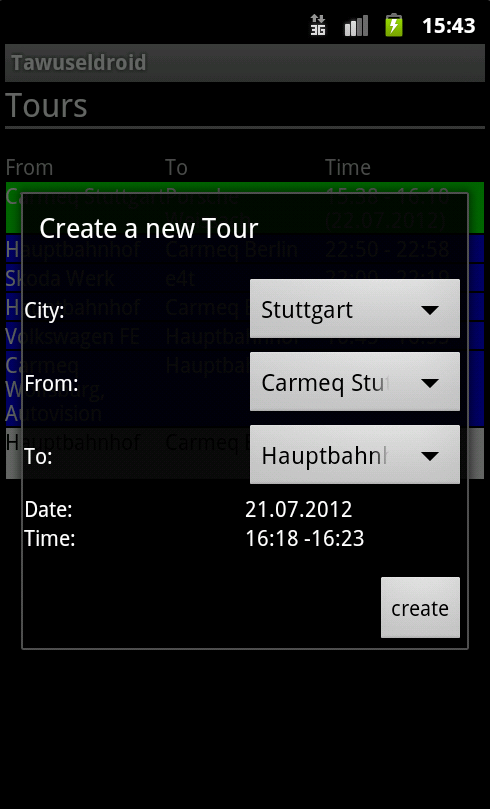
\includegraphics[width=4cm]{images/Tawuseldroid_create}
	\caption{create dialog}
	\label{img:AndCD}
\end{figure}

\begin{figure}[ht]
	\centering
	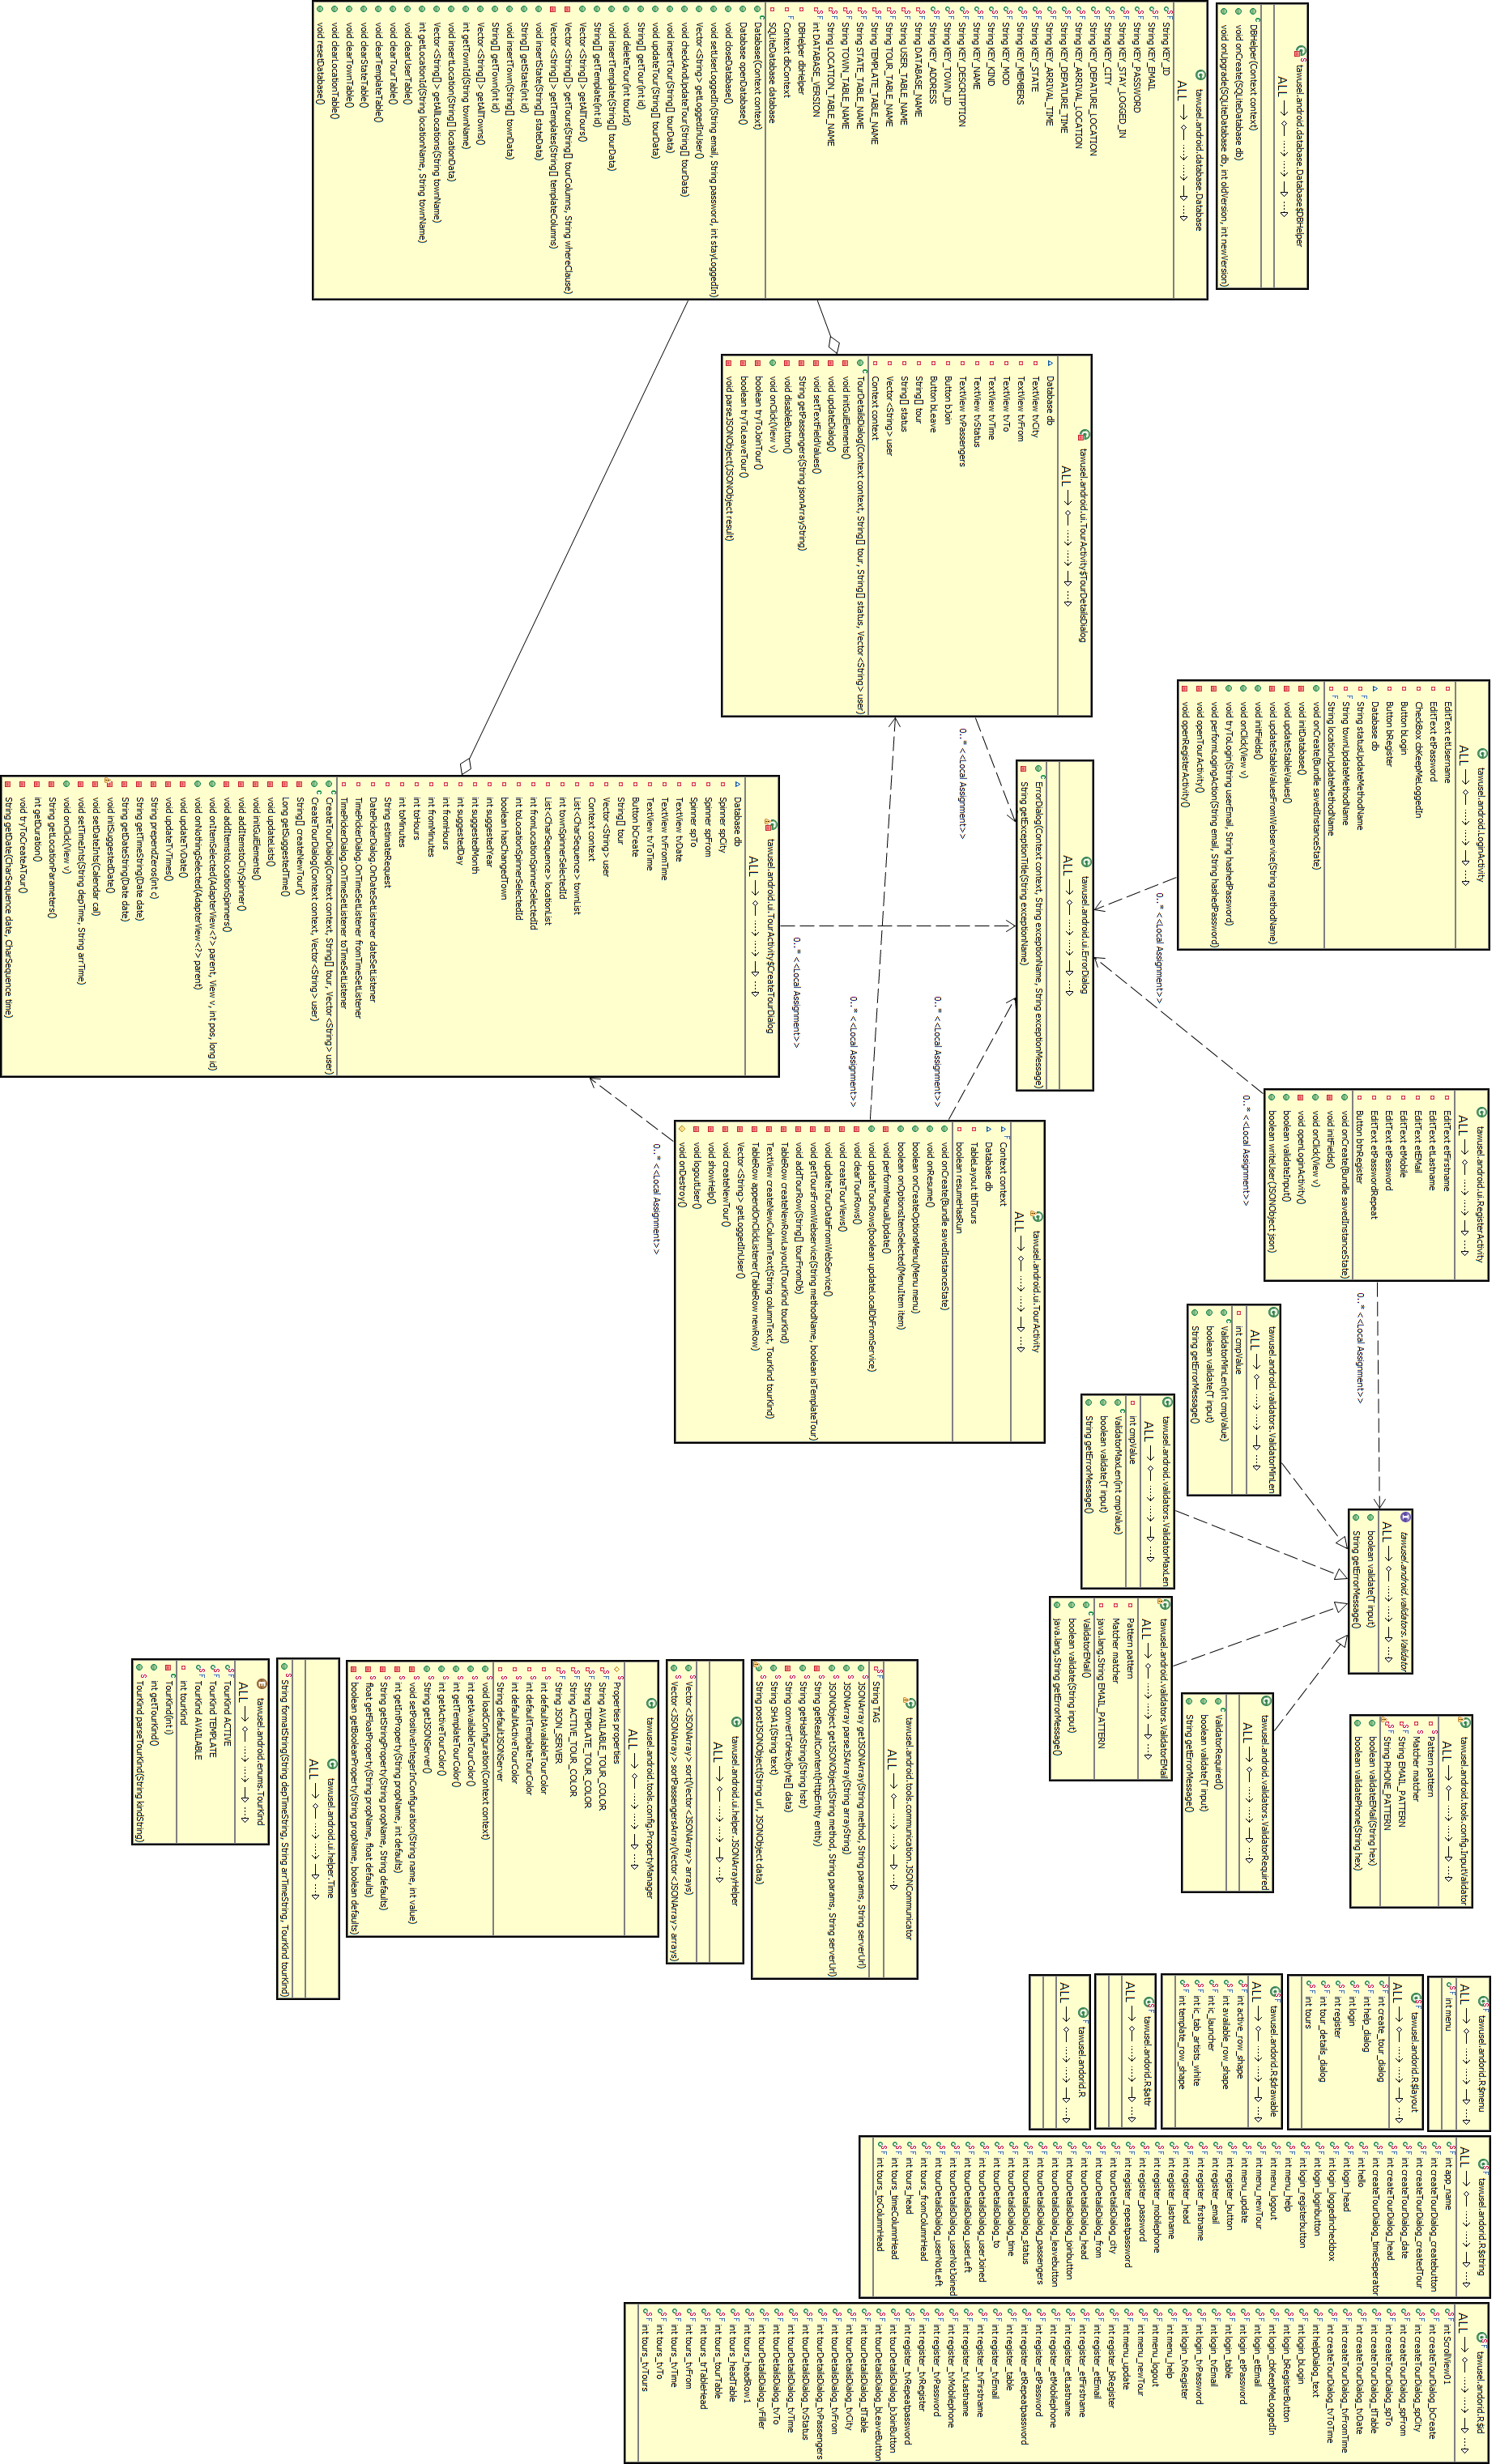
\includegraphics[height=.9\textheight]{images/Tawuseldroid_class}
	\caption{class diagram of the TaWusel android app}
	\label{img:AndCl}
\end{figure}

\chapter{User stories}\label{chp:US}
In this chapter yo will find the document which contains all sprint informations which arose from the project progress.

\clearpage
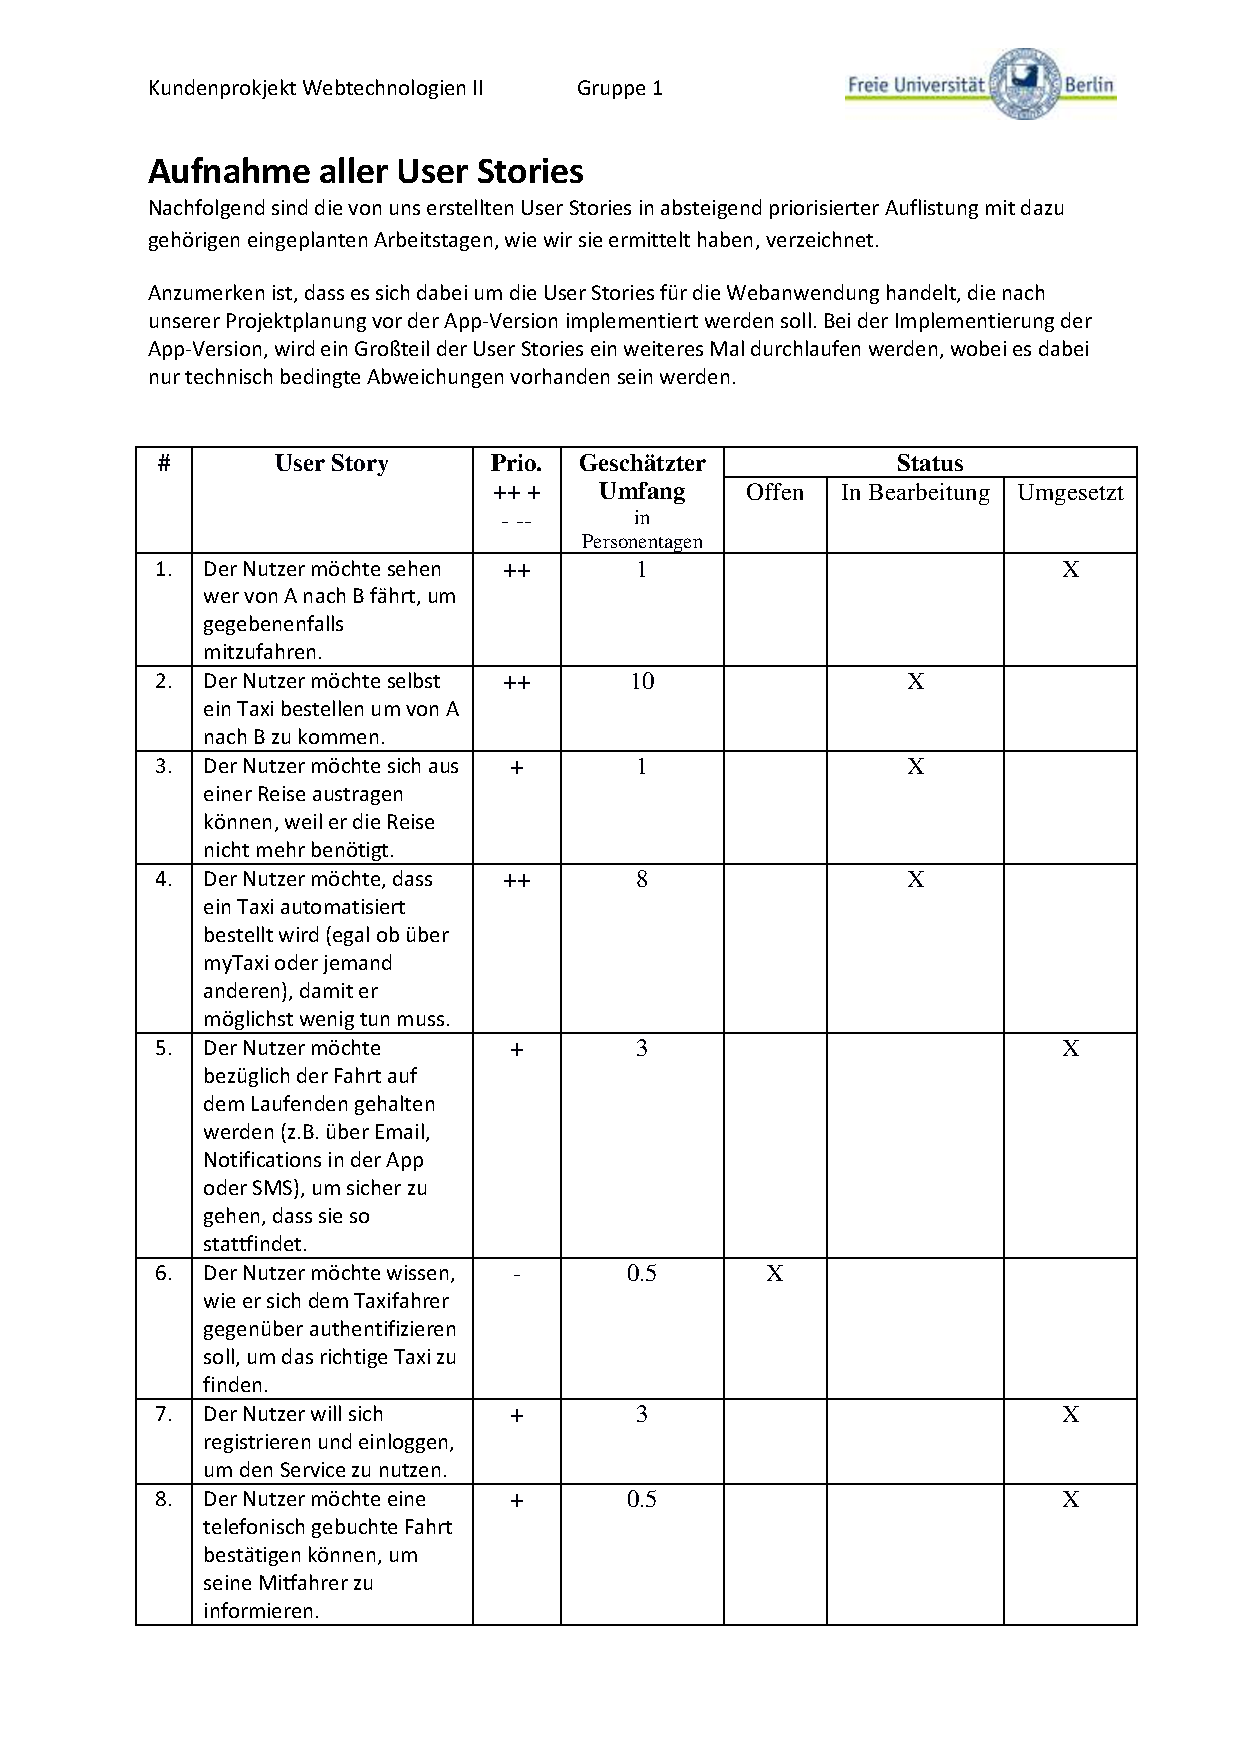
\includepdf[pages=-, pagecommand={\thispagestyle{fancy}}]{images/User_Stories.pdf}

	
	%literaturverzeichnis
%	\addcontentsline{toc}{chapter}{Literaturverzeichnis}
	
	%nicht-zitierte BibTeX-Eintr�ge anzeigen
%	\def\btxmastthesis{Ausarbeitung}
%	\def\btxvolumelong{Auflage}
%	\def\btxandlong{und}
%	\bibliographystyle{mygeralpha}
%	\bibliography{literatur}

\end{document}

